\chapter{Database Design I Samanfattning}

\textbf{Resorcess}
\begin{itemize}
    \item \url{https://www.w3schools.com/sql/}
    \item \url{https://www.mysql.com/}
    \item \url{https://erdplus.com/}
\end{itemize}


\newpage
\section{Ch1. Databases and Database Users}
\begin{itemize}
    \item \textit{Database}: A collection of related data.
    \item \textit{Data}: Known facts that can be recorded and have an implicit meaning.
    \item \textit{Mini-world}: Some part of the real world about which data is stored 
    in a database. For example, student grades and transcripts at a university.
    \item \textit{Database Management System (DBMS)}: A software package/ system to 
    facilitate the creation and maintenance of a computerized database.
    \item \textit{Database System}: The DBMS software together with the data itself. 
    Sometimes, the applications are also included.
\end{itemize}

\begin{figure}[!h]
    \centering
    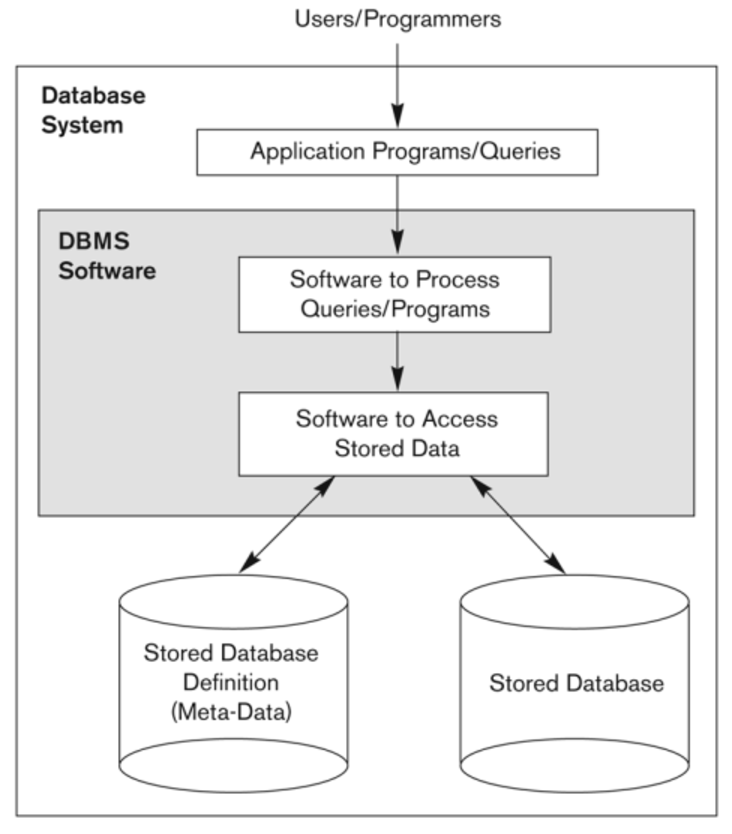
\includegraphics[width=12cm]{image/database-system.pdf}
    \caption{Database system}
\end{figure}

\newpage
\section{Ch3. Data Modeling Using the Entity-Relationship (ER) Model}
\begin{figure}[!h]
    \centering
    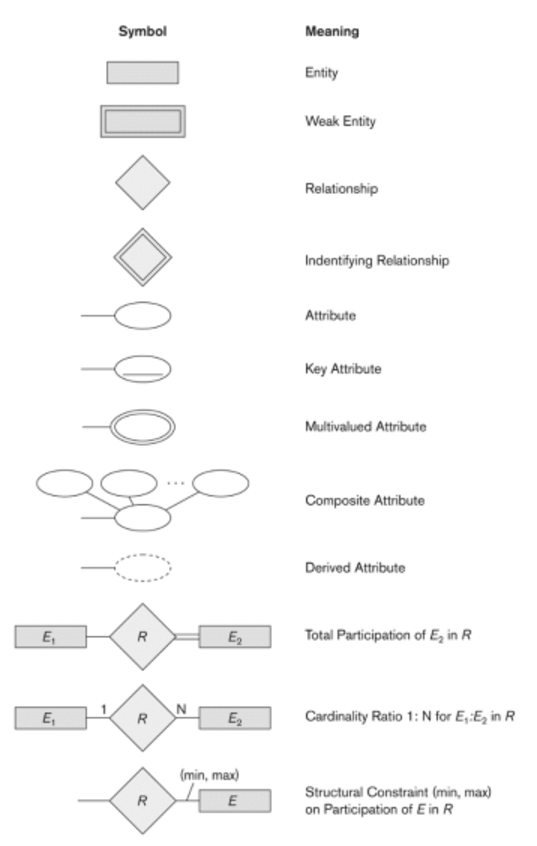
\includegraphics[width=10cm]{image/notation-er-diagrams.pdf}
    \caption{NOTATION ER Diagram}
\end{figure}

\newpage
\noindent\textbf{Definitions of ..}
\begin{itemize}
    \item \textit{Entity}: Entities are specific things or objects in the 
    mini-world that are represented in the database.
    \item \textit{Entity set}: Each entity type will have a collection of entities stored in the database
    \item \textit{Value sets}: Each simple attribute is associated with a value set
    \item \textit{Weak Entity}: dependencies on other entity to exist
    \item \textit{Relationship}: How entities are connected with one another
    \item \textit{Relationship types}: Identifies the relationship name and the participating entity types and also identifies certain relationship constraints
    \item \textit{Relationship Set}: The current set of relationship instances represented in the database
    \item \textit{Recursive relationship}: Both participations are same entity type in different roles
    \item \textit{Identifying Relationship}: Is the relationship for a entity to it's owner
    \item \textit{Attribute}: Data with the entity stores
    \item \textit{Simple Attribute}: Containing a single atomic value
    \item \textit{Key Attribute}: Uniq attributes, can be used as keys
    \item \textit{Multivalued Attributes}: Have multiple values like a list
    \item \textit{Composite Attribute}: composed of several components
    \item \textit{Derived Attributes}: Name(FirstName, MiddleName, LastName).
\end{itemize}

%Foreign keys
%constraints (key)

\newpage
\noindent\textbf{Relationship caractaristics}
\begin{itemize}
    \item Dubble line: Needs to have the relationship
    \item Single line: Can have the relationship
    \item 1: Only has one
    \item N: Many \underline{has} relationship (Used for one to many 1:N and N:1)
    \item M: Many relationship (Only used for many to many N:M and M:N)
    \item (1:1-samband): one to one
    \item (1:N-samband): one to many
    \item (N:M-samband): many to many 
    \item Doted key attribute: Is in combinations with the previus key
\end{itemize}

\begin{figure}[!h]
    \centering
    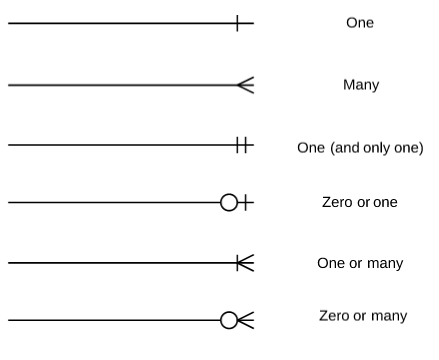
\includegraphics[width=8cm]{image/crow_foot.png}
    \caption{Crow foot notation}
\end{figure}


%When stating relationship one reads from left to right (EMMPLOYEE WORKS_FOR DEPARTMENT).
%crow feet. UML class diagrams
% weak entity the author matters
\newpage
\section{Ch4. Enhanced Entity-Relationship (EER) Modeling}
EER includes all modeling consents of basic ER, but also have additional concepts witch are:
\begin{itemize}
    \item \textit{subclasses/superclasses}: additional meaningful subgroups of its entities, (ex: EMPLOYEE is futher grouped into SECRETERY, ENGINEER, MANAGER)
    \item \textit{Specialization/generalization}: is the process of defining a set of subclasses of a superclass, (ex: {SECRETERY, ENGINEER, MANAGER} is spacialization of EMPLOYEE based upon job type)
    \begin{itemize}
        \item \textit{Disjointness Constraint}: an entity can be a member of at most one of the subclasses of the specialization
        \item \textit{Completeness Constraint}: Total specifies that every entity in the superclass must be a member of some subclass in the specialization/generalization
    \end{itemize}
    %\item \textit{categories (UNION types)}:
    %\item \textit{Attribute and relationship inheritance}:
\end{itemize} 

\begin{figure}[!h]
    \centering
    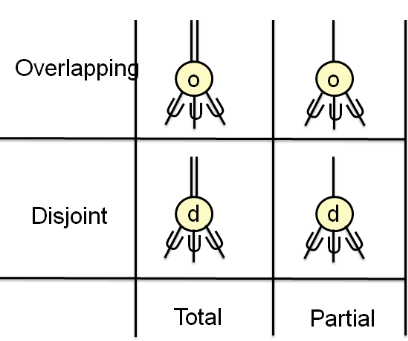
\includegraphics[width=8cm]{image/constraints_specialization-generalization.png}
    \caption{Overlapping, can be a member of multiple subclasses. Disjoint, can only be a member of at most one of the subclasses (Disjointness Constraint),  Total, it must be a member of at least one (Completeness constraint). Partial, don't need to belong to any of the subclasses}
\end{figure}


\newpage
\section{Ch5. The Relational Data Model and Relational Database Constraints}
\noindent\textbf{Definitions}
\begin{itemize}
    \item \textit{Schema}: Is the description of the relation
    \item \textit{Tuple}: is an ordered set of values (row)
    \item \textit{Domain}: each attribute has a domain or a set of valid values
    \item \textit{Relations}: Is a set of data (table)
\end{itemize}

\subsection{Constrains}
Constraints determine which values are permissible and 
which are not in the database
\begin{itemize}
    \item \textbf{Inherent or Implicit Constraints}: These are based on the data model itself. (E.g., relational model does not allow a list as a value for any attribute)
    \item \textbf{Schema-based or Explicit Constraints}: They are expressed in the schema by using the facilities provided by the model. (E.g., max. cardinality ratio constraint in the ER model) 
    \item \textbf{Application based or semantic constraints}: These are beyond the expressive power of the model and must be specified and enforced by the application programs. 
\end{itemize}

\subsubsection{Relational Integrity Constraints}
There are three main types of (explicit schema-based) 
constraints that can be expressed in the relational model:
\begin{itemize}
    \item \textit{Domain constraint}: \newline if one of the attribute values provided for the new tuple is not of the specified attribute domain
    \item \textit{Key constraints}: \newline if the value of a key attribute in the new tuple already exists in another tuple in the relation
    \item \textit{Referential integrity}: \newline if a foreign key value in the new tuple references a primary key value that does not exist in the referenced relation
    \item \textit{Entity integrity}: \newline if the primary key value is null in the new tuple
\end{itemize}

\newpage
\section{Ch.13 Normalization}
\href{https://www.youtube.com/watch?v=xoTyrdT9SZI}{Youtube tutorial}
The process of decomposing unsatisfactory "bad"
relations by breaking up their attributes into
smaller relations


\subsection{Anomalies}
Having redudent information creates some 
\begin{itemize}
    \item \textit{Insertion anomalies}: Can not Insertion unless there exist other data
    \item \textit{Deletion anomalies}: By deleting an objects other objects will be deleted 
    \item \textit{Modification/Update anomalies}: An update result in updating many other objects attribute
\end{itemize}

\textbf{EXAMPLE OF AN INSERT ANOMALY}
\begin{itemize}
    \item Consider the relation:
    \begin{itemize}
        \item  \begin{verbatim} EMP_PROJ(Emp#, Proj#, Ename, Pname, No_hours) \end{verbatim}
    \end{itemize}
    \item Insert Anomaly:
    \begin{itemize}
        \item Cannot insert a project unless an employee is
            assigned to it.
    \end{itemize}
\end{itemize}


\textbf{EXAMPLE OF AN DELETE ANOMALY}
\begin{itemize}
    \item Consider the relation:
    \begin{itemize}
        \item  \begin{verbatim} EMP_PROJ(Emp#, Proj#, Ename, Pname, No_hours) \end{verbatim}
    \end{itemize}
    \item Delete Anomaly:
    \begin{itemize}
        \item When a project is deleted, it will result in deleting
            all the employees who work on that project.
        \item Alternately, if an employee is the sole employee
            on a project, deleting that employee would result in
            deleting the corresponding project.
    \end{itemize}
\end{itemize}


\textbf{EXAMPLE OF AN UPDATE ANOMALY}
\begin{itemize}
    \item Consider the relation:
    \begin{itemize}
        \item  \begin{verbatim} EMP_PROJ(Emp#, Proj#, Ename, Pname, No_hours) \end{verbatim}
    \end{itemize}
    \item Update Anomaly:
    \begin{itemize}
        \item Changing the name of project number P1 from
            “Billing” to “Customer-Accounting” may cause this
            update to be made for all 100 employees working
            on project P1.
    \end{itemize}
\end{itemize}
Note that it is not the relation \textit{EMP\_PROJ}
who has the Anomaly, it is \textit{PROJ}.

\subsection{Normal forms}
\href{https://www.lifewire.com/database-normalization-basics-1019735}{Database Normalization Basics}
Condition using keys and FDs of a relation to
certify whether a relation schema is in a particular
normal form
\begin{itemize}
    \item 1NF: All attributes depend on the key. \href{https://www.youtube.com/watch?v=mUtAPbb1ECM}{Explanation 1NF}. 
    \begin{itemize}
        \item Requirements:
        \begin{enumerate}
            \item Each table cell should contain a single value, no multi-value or composite attributes.
            \item Columns which contain sets of values or nested records are not allowed.
        \end{enumerate}
        \item Steps:
        \begin{itemize}
            \item Eliminate duplicative columns from the same table.
            \item Create separate tables for each group of related data and identify each row with a unique column or set of columns (the primary key).
        \end{itemize}
    \end{itemize}
    \item 2NF: All attributes depend on the whole key. In other words
    there should not be any partial dependencies, meaning that a attribute
    depends on a key constructing a composite primary key. There for dose all 
    attribute on the entire composite key. This is especially relevant for 
    many to many reflations since a attribute can depend only on one foreign key 
    but the primary key is the composition of the two foreign keys.
    \href{https://www.youtube.com/watch?v=R7UblSu4744}{Explanation 2NF}.
    \begin{itemize}
        \item Requirements:
        \begin{enumerate}
            \item Meet the requirements of 1NF.
            \item Not have duplicates in any table, if present, normalize further that table. Create relations between these new tables that are created and use foreign keys between them in order to indicate a relation is present. 
        \end{enumerate}
        \item Steps
        \begin{itemize}
            \item Meet all the requirements of the first normal form.
            \item Remove subsets of data that apply to multiple rows of a table and place them in separate tables.
            \item Create relationships between these new tables and their predecessors through the use of foreign keys.
        \end{itemize}
    \end{itemize}
    \item 3NF: All attributes depend on nothing but the key. In other words 
    does there not exist any attribute with depend on a other attribute or key
    witch is not the primary key.
    \href{https://www.youtube.com/watch?v=aAx_JoEDXQA}{Explanation 3NF}.
    \begin{itemize}
        \item Requirements:
        \begin{enumerate}
            \item Meet the requirements of 2NF.
            \item Have no transitive functional dependencies.
        \end{enumerate}
        \item Steps:
        \begin{itemize}
            \item Meet all the requirements of the second normal form.
            \item Remove columns that are not dependent upon the primary key.
        \end{itemize}
    \end{itemize}
    \item 4NF: (will not look at)
    \item BCNF: (will not look at)
\end{itemize}

primary key, full functional dependency
Functional Dependencies FD

Transmit dependencies FD1 FD2 FD3 ..

%step 7  wont look at
\newpage
\section{Ch.9}
\textbf{ER-to-Relational Mapping Algorithm}
\begin{itemize}
    \item Step 1: Mapping of Regular Entity Types
    \item Step 2: Mapping of Weak Entity Types
    \item Step 3: Mapping of Binary 1:1 Relation Types
    \item Step 4: Mapping of Binary 1:N Relationship Types.
    \item Step 5: Mapping of Binary M:N Relationship Types.
    \item Step 6: Mapping of Multi-valued attributes.
    \item Step 7: Mapping of N-ary Relationship Types.
\end{itemize}

\noindent\textbf{Mapping EER Model Constructs to Relations}
\begin{itemize}
    \item Step 8: Options for Mapping Specialization or Generalization.
    \item Step 9: Mapping of Union Types (Categories).
\end{itemize}

\newpage
\section{Ch.6 SQL}
\subsection{Terminology}
\begin{itemize}
    \item \textit{Table}
    \item \textit{Row}
    \item \textit{Column}
    \item \textit{SQL schema}: Identified by a schema name and includes an authorization identifier and descriptors
for each element
    \item \textit{Schema elements}: includes the document element (the top-level element) in a schema definitionTables, constraints, views, domains, and other 
constructs
    \item \textit{Catalog}: Named collection of schemas in an SQL environment.
    \item \textit{Base tables (base relations)}: Relation and its tuples are actually created and 
        stored as a file by the DBMS
    \item \textit{Virtual relations (views)}: Created through the CREATE VIEW statement. 
        Do not correspond to any physical file.
    \item \textit{Aliases}: a alternative name to the relation (table). Declared by \textbf{AS}
    \item \textit{Tuple}: a row value
\end{itemize} 
%Table, row, and column used for relational model terms relation, tuple, and attribute.

\subsection{SQL types}
\begin{itemize}
    \item Numeric
    \begin{itemize}
        \item Integer numbers: INTEGER, INT, SMALLINT
        \item Floating-point: FLOAT or REAL, DOUBLE PRECISION
    \end{itemize}
    \item Character-string
    \begin{itemize}
        \item Fixed length: CHAR(n), CHARACTER(n)
        \item Varing lenght: VARCHAR(n), CHAR VARYING(n), CHARACTER VARYING(n)
    \end{itemize}
    \item Bit-string
    \begin{itemize}
        \item Fixed lenght: BIT(n)
        \item Varying length: BIT VARYING(n)
    \end{itemize}
    \item Boolean
    \begin{itemize}
        \item TRUE or FALSE or NULL
    \end{itemize}
    \item DATE
    \begin{itemize}
        \item YEAR, MONTH, DAY
    \end{itemize}
    \item Additional data types 
    \begin{itemize}
        \item Timestamp: DATE, TIME
    \end{itemize}
    \item INTERVAL
\end{itemize}

\subsection{SQL examples}
\begin{verbatim}
    -- Creating tables

    CREATE TABLE T1 (C1 VARCHAR(20), C2 VARCHAR(10), C3 INT);
    INSERT INTO T1 VALUES ("a", "x", 1);
    INSERT INTO T1 VALUES ("a", "y", 5);
    INSERT INTO T1 VALUES ("b", "z", 2);
    INSERT INTO T1 VALUES ("c", "z", 2);
    INSERT INTO T1 VALUES ("d", "u", 3);

    CREATE TABLE T2 (C1 VARCHAR(20), C2 VARCHAR(10), C3 INT);
    INSERT INTO T2 VALUES ("a", "z", 4);
    INSERT INTO T2 VALUES ("a", "x", 3);
    INSERT INTO T2 VALUES ("b", "z", 2);
    INSERT INTO T2 VALUES ("b", "x", 1);
    INSERT INTO T2 VALUES ("c", "u", 2);

    -- Select statements
    
    SELECT COUNT(*)
    FROM T1, T2; 
    -- T1 and T2 have 5 rows each there for is the result 5*5=25

    SELECT Count(*)
    FROM T1, T2
    WHERE T1.C1=T2.C1; 
    -- 2+2+2+1=7

    SELECT DISTINCT T1.C1
    FROM T1, T2
    WHERE T1.C2=T2.C2;
    -- [a,b,c,d] (if the first is distinct) c,b,a,d (is the output)

    SELECT T1.C2, AVG(T1.C3*T2.C3)
    FROM T1, T2
    WHERE T1.C2 = T2.C2
    GROUP BY T1.C2;
    -- [[u, 6],[x, 2],[z, 6]]

    SELECT T1.C2, SUM(T1.C3*T2.C3)
    FROM T1, T2
    WHERE T1.C2 = T2.C2
    GROUP BY T1.C2
    HAVING SUM(T1.C3*T2.C3)>10  
    -- [z, 24] since u=6<10 and x=4<10 and z=2*4+2*2+2*4+2*2=24 

    SELECT count(*)
    FROM T1 INNER T2 ON (T1.C1 = T2.C1);  
    -- Is an incorrect sql statement INNER JOIN is probably the right way

    SELECT T1.C1
    FROM T1 INNER JOIN T2 ON (T1.C1 = T2.C1)
    WHERE (T1.C3>2);
    -- [a, a] since there is only one a in T1 where T1.C3>2 and there is 2 a in T2

    SELECT T2.C2
    FROM T1 LEFT OUTER JOIN T2 ON (T1.C2 = T2.C2);
    -- [x,x,NULL,z,z,z,z,u] the NULL comes from T1.C2="y"

\end{verbatim}
\begin{figure}[!h]
    \centering
    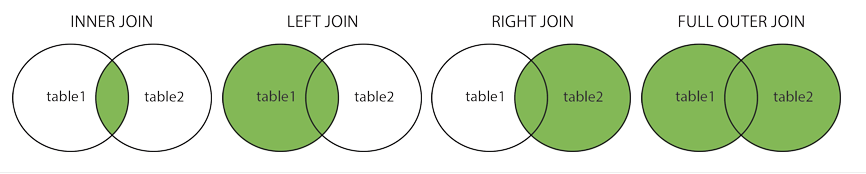
\includegraphics[width=12cm]{image/sql_joins.png}
    \caption{SQL JOIN statements}
    \label{fig:sql_joins}
\end{figure}


\subsection{Constraints}
\begin{itemize}
    \item \textbf{Key} constraint: A primary key value cannot be duplicated.
    \item \textbf{Entity Integrity} Constraint: A primary key value cannot be null. 
    \item \textbf{Referential integrity} constraints : The “foreign key “ must have a value that is already present as a primary key, or may be null.
\end{itemize}

% transaction control with sql
% we need to pick with relation to start with (the realation should not point to any other)
% To types of table (base table and virtual relation)
% Populate: insert data to the table so it hase some data. 
% types of keys, candidate key
% key constraint: A primary key value cannot be duplicated
% base table?
% join creates new table "result" from when the tables follows the define roolse/reasrch
% the output will be of a table

\newpage
\section{Ch.20 Transaction}
\textbf{Terminology}
\begin{itemize}
    \item \textit{Transaction}: Describes local unit of database processing
    \item \textit{Transaction processing systems}: Systems with large databases and hundreds of concurrent users. Require high availability and fast response time
    \item \textit{Single-user DBMS}: At most one user at a time can use the system
    \item \textit{Multi-user DBMS}: Many users can access the system (database) concurrently
    \item \textit{Multiprogramming}: Executes commands from one process, then suspends that process and executes commands from another process, etc.
    \item \textit{Interleave processing}: Interleaving is a process or methodology to make a system more efficient, fast and reliable by arranging data in a noncontiguous manner.
    \item \textit{Parallel processing}: Parallel computing is a type of computation in which many calculations or processes are carried out simultaneously.
    \item \textit{Read-only transaction}: (read\_item(X))
    \item \textit{Read-write transaction}: (read\_item(X) and write\_item(X))
    \item \textit{Read set of transaction}: Set of all items read
    \item \textit{Write set of a transaction}: Set of all items written
    \item \textit{Concurrency control}: Transactions submitted by various users may execute concurrently
    \item \textit{The lost update problem}: Occurs when two transactions that access the same database items have operations interleaved
    \url{https://www.youtube.com/watch?v=C_J6K8DodS8}
    \item \textit{The temporary update problem}: Reading and updating from one transaction then read and write from another transaction. Then when reading another item we go back to the previous state. The problem is the dirty read of write then read from one transaction to another \ref{fig:temporary_update_problem}. 
    \url{https://www.youtube.com/watch?v=d4Ziyuri0L0}
    \item \textit{The incorrect summary problem}: $T_3$ reads X after N is subtracted and reads Y before N is added; a wrong summary is the result (off by N) \ref{fig:incorrect_summary_problem}.
    \url{https://www.youtube.com/watch?v=IIcR3G5w4ZI}
    \item \textit{The unrepeatable read problem}: Transaction T reads the same item twice. Value is changed by another transaction T' between the two reads. T receives different values for the two reads of the same item.
    \item \textit{Recovery}: 
    \begin{itemize}
        \item \textit{Committed transaction}: Effect recorded permanently in the database
        \item \textit{Aborted transaction}: Does not affect the database
        \item \textit{Transaction faliures}:
        \begin{itemize}
            \item \textit{Computer failure}
            \item \textit{Transaction or system error}
            \item \textit{Local error or exception conditions detected by the transaction}
        \end{itemize}
    \end{itemize}
    \item \textit{Transaction and System Concepts}
    \begin{itemize}
        \item BEGIN\_TRANSACTION
        \item READ or WR
        \item END\_TRANSACTION
        \item COMMIT\_TRANSACTION
        \item ROLLBACK (or ABORT)
    \end{itemize}
    \item \textit{system log}: System log keeps track of transaction operations
    \item \textit{ACID properties}
    \begin{itemize}
        \item \textit{Atomicity}: Transaction performed in its entirety or not at all
        \item \textit{Consistency preservation}: Takes database from one consistent state to another
        \item \textit{Isolation}: Not interfered with by other transactions
        \item \textit{Durability or permanency}: Changes must persist in the database
    \end{itemize}
    \item \textit{Schedule}: (or history) Order of execution of operations from all transactions
    \item \textit{Serializable schedules}: Places simultaneous transactions in series
    \item \textit{serial schedules}: Everything in series results limit of concurrency
    \item \textit{Conflict equivalence}: Relative order of any two conflicting operations is the same in both schedules.
    \item \textit{DBMS enforces protocols}: Set of rules to ensure serializability.
\end{itemize}

\subsubsection{Other SQL syntax}
\textbf{Set operations}
\begin{itemize}
    \item UNION: The UNION operator is used to combine the result-set of two or more SELECT statements.
    \item EXCEPT: The SQL EXCEPT clause/operator is used to combine two SELECT statements and returns rows from the first SELECT statement that are not returned by the second SELECT statement
    \item INTERSECT: The INTERSECT clause in SQL is used to combine two SELECT statements but the dataset returned by the INTERSECT statement will be the intersection of the data-sets of the two SELECT statements
\end{itemize}

\textbf{Substring Pattern Matching}
\begin{itemize}
    \item LIKE: The LIKE operator is used in a WHERE clause to search for a specified pattern in a column.
    \item BETWEEN: The BETWEEN operator selects values within a given range.
\end{itemize}

\textbf{Aliasing}

%image from slide 20-19
\subsection{Transaction Support in SQL}
\begin{itemize}
    \item No explicit Begin\_Transaction statement
    \item Every transaction must have an explicit end statement
    \begin{itemize}
        \item COMMIT
        \item ROLLBACK
    \end{itemize}
    \item Access mode is READ ONLY or READ WRITE
    \item Diagnostic area size option: Integer value indicating number of conditions held 
simultaneously in the diagnostic area
    \item Isolation level option
    \begin{itemize}
        \item Dirty read
        \item Nonrepeatable read
        \item Phantoms
    \end{itemize}
\end{itemize}

\newpage
\begin{appendices}
\begin{figure}[!h]
    \centering
    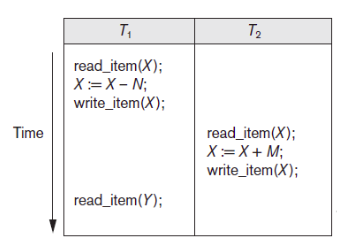
\includegraphics[width=12cm]{image/temporary_update_problem.png}
    \caption{Temporary update problem}
    \label{fig:temporary_update_problem}
\end{figure}
\begin{figure}[!h]
    \centering
    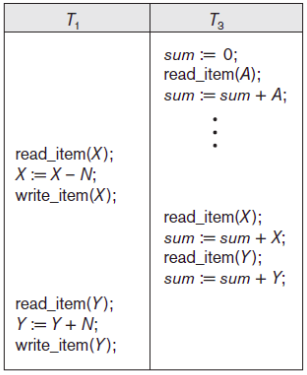
\includegraphics[width=12cm]{image/incorrect_summary_problem.png}
    \caption{Incorrect summary problem}
    \label{fig:incorrect_summary_problem}
\end{figure}
\end{appendices}
